\documentclass[UTF8, 12pt]{ctexart}

\usepackage{amsmath}

\usepackage{geometry}
\geometry{a4paper, scale = 0.9} % a4纸, 版心占页面长度的比例为0.9

\usepackage{enumitem} % itemize, 列表

\usepackage{graphicx}

\begin{document}

	\noindent
	多级放大电路的一般问题 :

	对耦合电路的要求 : 各级静态工作点合适, 不失真, 减小小信号的损失

	阻容耦合 :
	\begin{itemize}[leftmargin = 4em]
		\item 静态工作点互不影响, 交流损失小
		\item 不能放大变化缓慢的信号, 不便于集成
	\end{itemize}

	直接耦合($ U_ {CE1} = U_{BE2}$) :
	\begin{itemize}[leftmargin = 4em]
		\item 频率特性好, 可以放大缓慢的信号, 可以集成
		\item 各级工作点影响, 零点漂移($ U_{i} = 0 $ 时, 输出电压无规则缓慢漂动, 主要由温度变化引起, 直流负反馈/差分放大可以抑制零漂)
		\item 可以NPN管和PNP管搭配的方式, 避免集电极电位升高
	\end{itemize}

	分析 :
	\begin{itemize}[leftmargin = 4em]
		\item 直流 : 画直流通路, 从输入到输出分析
		\item 交流 : 将后一级的输入电阻作为这一级的负载考虑(这一级的公式中的 $ R_{L} $ 换成下一级的 $ R_{i} $), 电压增益为每一级电压增益的乘积, 输入电阻为第一级的输入电阻, 输出电阻为最后一级的输出电阻
		\item 注意 : 输入/输出电阻如果和信号源内阻有关, 则内阻为上一级的输出电阻; 计算电压增益一定要记得下一级的输入电阻
	\end{itemize}

	~

	\noindent
	集成运算放大电路 : 符号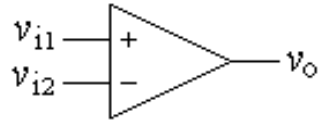
\includegraphics[scale = 0.2]{03/集成运算放大器符号.png}, +为同相输入端, -为反相输入端

	电压传输特性($ u_{p}, u_{n} $ 分别为同相, 反相输入端电位, 在线性区有 $ u_{o} = A_{od}(u_{p}-u_{n}) $, $ A_{od} $ 称为开环差模放大倍数) :

	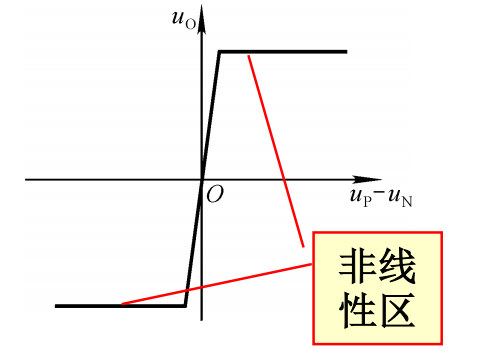
\includegraphics[scale = 0.4]{03/集成运算放大器电压传输特性.png}

	~

	\noindent
	差分放大电路 :

	(1). 基本差分放大电路 :

	电路图 :

	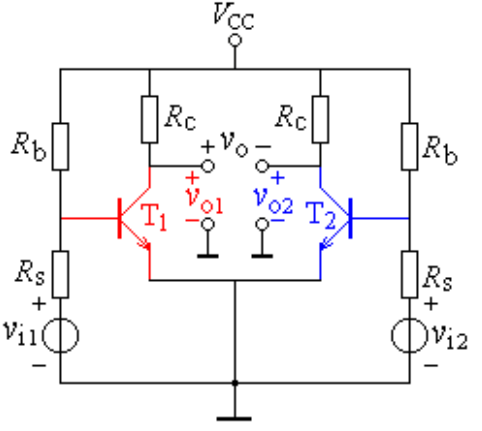
\includegraphics[scale = 0.4]{03/基本差分放大电路电路图.png}

	特点与分析 :
	\begin{itemize}[leftmargin = 4em]
		\item 电路对称, 三极管参数相同
		\item 抑制零漂 : 输入为0的时候输出也为0
		\item 共模信号(幅度极性相同的信号) : $ v_{oc} = 0 $
		\item 差模信号(幅度相同, 极性相反) : $ v_{od} = 2v_{o1} $
		\item 问题 : 没有调零, 半边没有抑制零漂
	\end{itemize}

	(2). 长尾式差分放大电路 :

	电路图 :

	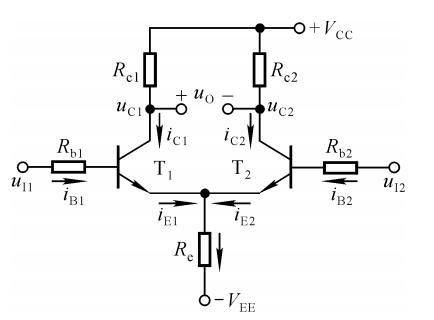
\includegraphics[scale = 0.4]{03/长尾式差分放大电路电路图.png}

	差模交流通路 :

	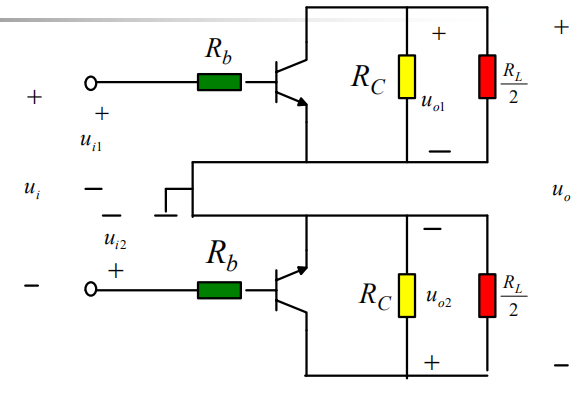
\includegraphics[scale = 0.4]{03/长尾式差分放大电路差模输入交流通路.png} 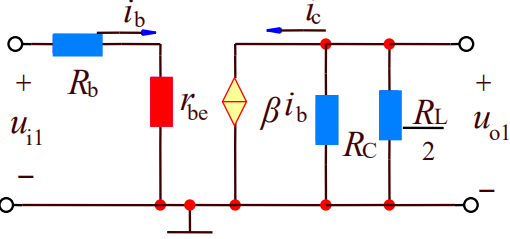
\includegraphics[scale = 0.4]{03/长尾式差分放大电路差模输入交流通路(2).png}

	共模交流通路 :

	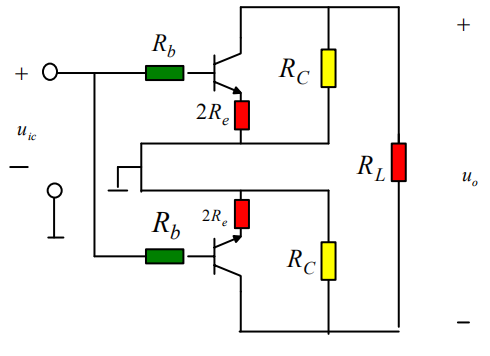
\includegraphics[scale = 0.4]{03/长尾式差分放大电路共模输入交流通路.png} 

	分析 :
	\begin{itemize}[leftmargin = 4em]
		\item 直流 : $ I_{B} = \frac{|V_{EE}-U_{BE}|}{R_{b}+(1+\beta)2R_{e}} $
		\item 差模 : 差模输入变化, $ i_{Re} $ 不变, $ R_{e} $ 对差模信号相当于短路. $ A_{ud} = \frac{u_{o}}{u_{i}} = \frac{u_{o1}}{u_{i1}} = -\frac{\beta(R_{c} \parallel \frac{R_{L}}{2})}{R_{b}+r_{be}}, R_{id} = 2(R_{b}+r_{be}), r_{od} = 2R_{c} $
		\item 共模 : E点两端等电位, 将其断开. $ A_{uc} = 0, R_{ic} = \frac{1}{2}(R_{b}+r_{be}+(1+\beta)2R_{e}), R_{oc} = 2R_{c} $
		\item 共模抑制比 : $ K_{CMR} = |\frac{A_{ud}}{A_{uc}}| $
		\item 单端输出($ R_{c1} $ 两端并联 $ R_{L} $, $ R_{c2} $ 两端没有) : 差模 $ A_{uc} = \pm \frac{\beta(R_{c} \parallel R_{L})}{2(R_{b}+r_{be})} $, 共模 $ A_{uc} = -\frac{\beta(R_{c} \parallel R_{L})}{R_{b}+r_{be}+(1+\beta)2R_{e}} $ 
	\end{itemize}

	(3). 恒流源式差分放大电路 :

	电路图 :

	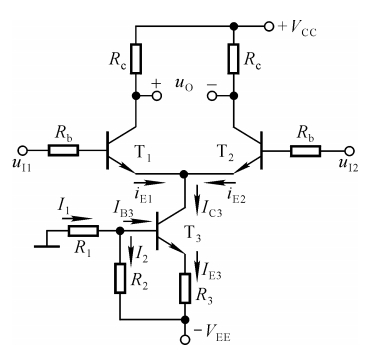
\includegraphics[scale = 0.4]{03/恒流源式差分放大电路电路图.png}

	分析 :
	\begin{itemize}[leftmargin = 4em]
		\item 直流 : $ U_{R2} = \frac{R_{2}}{R_{1}+R_{2}}V_{EE}, I_{C3} \approx I_{E3} = \frac{U_{R2}-U_{BE3}}{R_{3}}, I_{C1} = I_{C2} \approx \frac{I_{C3}}{2} $
		\item 改进 : E点加调零电位器, 场效应管
	\end{itemize}

	~

	\noindent
	电流源电路 :

	基本电流源($ T_{1} $ 的负载变化, $ I_{C1} = I_{R} $ 保持不变) :

	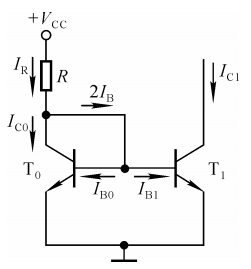
\includegraphics[scale = 0.4]{03/基本电流源电路图.png}

	比例电流源($ I_{C1} \approx \frac{R_{e0}}{R_{e1}}I_{R} $) :

	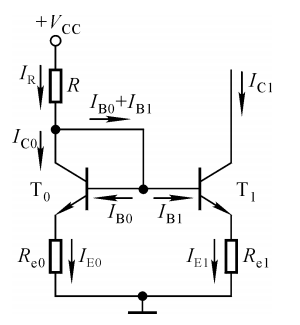
\includegraphics[scale = 0.4]{03/比例电流源电路图.png}

	~

	\noindent
	集成运放性能指标 :

	静态指标 :
	\begin{itemize}[leftmargin = 4em]
		\item 输入失调电压 :输入电压为0时,  为使输出电压为0, 在输入端加的补偿电压
		\item 输入失调电流 :输入电压为0时,  差分输入级的差分对管基极电流之差
		\item 输入偏置电流 : 运放两个输入端的偏置电流的平均值
		\item 输入失调电压温漂、输入失调电流温漂 : 规定的温度范围内, 输入失调电压随温度的变化量与温度的变化量之比
		\item 最大差模输入电压 :输入端能承受的最大差模输入电压,  超过此电压会反向击穿
		\item 最大共模输入电压 :正常工作情况下共模输入电压的允许范围, 超过此电压会失去共模抑制能力
	\end{itemize}

	动态指标 :
	\begin{itemize}[leftmargin = 4em]
		\item 开环差模放大倍数 :无外加反馈的情况下,  输出电压变化量与输入电压变化量之比
		\item 差模输入电阻, 共模抑制比 : 和差分电路一样
		\item -3dB带宽 : 差模电压放大倍数在高频段下降3dB所定义的带宽
		\item 单位增益带宽 : 开环差模放大倍数下降到1时对应的频率
	\end{itemize}

	理想运放条件 :
	\begin{itemize}[leftmargin = 4em]
		\item 开环差模放大倍数无穷大
		\item 差模输入电阻无穷大
		\item 输出电阻为0
		\item -3dB带宽足够宽
		\item 共模抑制比足够大
	\end{itemize}
	

\end{document}